\documentclass[../classical_mechanics.tex]{subfiles}

\begin{document}

    % TODO: add an interlude on 3D spherical and cylindrical coordinates

    \section{Moments}\label{sec:moments}
        \paragraph{}
        When dealing with problems involving rotation, we have mechanical quantities which are analogous to ones used to solve linear problems.
        We have seen a few of these before: angular velocity $\omega=v_\theta/r$, angular acceleration $\alpha=a_\theta/r$ (for circular motion), and moment of inertia $I=mr^2$.
        As we can see, the definitions of these quantities all involve the analogous linear quantity and the distance from the origin $r$.
        Quantities that involve the \textit{product} of a linear quantity with the radius are called \textbf{moments}.
        Moments we have seen already are the center of mass, which is the first moment of mass (sum of $mr$) normalised by the total mass, and the moment of inertia, which is the second moment of mass (mass multiplied by $r^2$)
        In this chapter we will introduce two more moments: torque --- the moment of force --- and angular momentum --- the moment of momentum.
        When vector quantities like force and momentum are involved, moments are defined using the cross product.
        \begin{definition}
            \textbf{Angular Momentum} is defined as the first moment of momentum.
            \begin{equation}
                \vec{L}=\vec{r}\times\vec{p}=m\vec{r}\times\vec{v}.
            \end{equation}
        \end{definition}
        Note that because the cross product is antisymmetric, the order of $\vec{r}$ and $\vec{p}$ matters!
        The motivation for introducing angular momentum will become clear in the next section. 

    \section{Central Forces}\label{sec:central-forces}
        \paragraph{}
        We will now examine a very special type of force.
        These forces have many useful properties which make solving problems involving them a lot simpler.
        \begin{definition}
            A \textbf{central force} is a force which acts along the radial direction and only depends on the radial distance $r$.
            Central forces thus have the form
            \begin{equation}
                \vec{F}=F(r)\uvec{r}.
            \end{equation}
            If $F(r)<0$, the force is attractive, and if $F(r)>0$, the force is repulsive.
        \end{definition}
        We have seen one example of a central force already, the universal law of gravitation.
        Another example is Coulomb's law.

        \paragraph{}
        Motion under a central force obeys the following rules:
        \begin{itemize}
            \item The motion is confined to a plane.
            \item The angular momentum is conserved ($\dv{\vec{L}}{t}=0$).
            \item The position vector sweeps out equal area in equal time.
        \end{itemize}
        
        \paragraph{}
        Let's prove that angular momentum is conserved under the influence of a central force.
        Looking at the derivative, we get
        \begin{align}
            \dv{\vec{L}}{t}&=\dv{}{t}(\vec{r}\times\vec{p})\\
            &=\dv{\vec{r}}{t}\times\vec{p}+\vec{r}\times\dv{\vec{p}}{t}\\
            &=\vec{v}\times m\vec{v}+\vec{r}\times F(R)\uvec{R}\\
            &=0.
        \end{align}
        Therefore, $\vec{L}$ is constant over time, it is conserved.

        \paragraph{}
        By definition, $\vec{L}$ is perpendicular to $\vec{r}$.
        We can also see this by taking the dot product of $\vec{L}$ with the position vector:
        \begin{equation}
            \vec{r}\cdot\vec{L}=\vec{r}\cdot(\vec{r}\times\vec{p})=\vec{p}\cdot(\vec{r}\times\vec{r})=0.
        \end{equation}
        Since $\vec{L}$ is constant, this implies that $\vec{r}$ is confined to the plane perpendicular to $\vec{L}$.
        
        \paragraph{}
        Because of this, it is convenient to use cylindrical coordinates with the plane $z=0$ as the plane of motion.
        Using equation~\ref{} (note that $\dot{z}=0$) and the cross products between unit vectors, we get
        % TODO: add reference to velocity in cylindrical coordinates here
        \begin{align}
            \vec{L}&=m\vec{r}\times\vec{v}\\
            &=mR\uvec{R}\times(\dot{R}\uvec{R}+R\dot{\theta}\uvec{\theta})\\
            &=mR^2\dot{\theta}\khat\label{eq:angular-momentum-theta-dot}\\
            &=mh\khat.
        \end{align}
        In the last line we have defined $h=R^2\dot{\theta}$.
        This is the \textbf{specific angular momentum} (angular momentum normalised by mass), and is useful in some problems.

        Finally, we will prove the last fact about motion under central forces, the law of equal areas, which is a more general version of Kepler's second law of planetary motion.
        Consider an object on a curved path at two points separated by a small time interval $\dd{t}$.
        \begin{figure}[H]
            \centering
            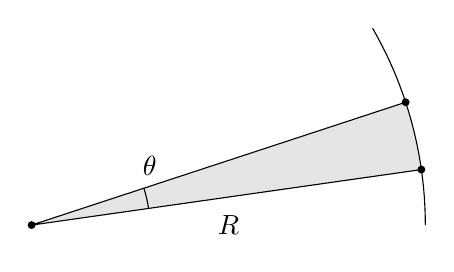
\begin{tikzpicture}[scale=5]
                \fill[fill=black!10,rotate=8] (0,0) -- (1,0) arc [radius=1, start angle=0, end angle=10.1] -- cycle;
                \draw[rotate=8] (0.3,0) arc [radius=0.3, start angle=0, end angle=10.1];
                \draw (1,0) arc [radius=1, start angle=0, end angle=30];
                \draw (0,0) -- (0.95,0.312) (0.99,0.141) -- (0,0);
                \fill (0.95,0.312) circle [radius=0.01];
                \fill (0.99,0.141) circle [radius=0.01];
                \fill (0,0) circle [radius=0.01];
                \node at (0.3,0.15) {$\dd{\theta}$};
                \node at (0.5,0) {$R$};
            \end{tikzpicture}
        \end{figure}
        The shaded arc is approximately a triangle, so the area get closer and closer to $A=\frac{1}{2}R^2\dd{\theta}$ as $\dd{t}\to0$.
        Therefore, we have
        \begin{equation}
            \dv{A}{t}=\frac{1}{2}R^2\dv{\theta}{t}=\frac{1}{2}h=\text{const}.
        \end{equation}
        So the rate of area swept out over time is constant.

        \paragraph{}
        What does motion under a central force look like?
        By Newton's second law, we know that
        \begin{equation}\label{eq:central-force-eom}
            a_R=\ddot{R}-R\dot{\theta}^2=\frac{F(R)}{m}.
        \end{equation}
        Substituting in the specific angular momentum, we get
        \begin{equation}
            \ddot{R}-\frac{h^2}{R^3}=\frac{F(R)}{m}.
        \end{equation}
        This is the differential equation we need to solve for any central force problem.
        \begin{example}
            Prove Kepler's third law: the square of a planet's orbital period is proportional to the cube of the semi-major axis of its orbit.

            \paragraph{}
            Planets move according to the universal law of gravitation, which is
            \begin{equation}
                \vec{F}=-\frac{GMm}{R^2}\uvec{R}.
            \end{equation}
            We will make an approximation and assume that the sun is fixed at the origin and the planets orbit in circular orbits.
            In reality, the a given planet and the sun orbit their common centre of mass in elliptical paths, but the difference is very small making this approximation makes the problem much simpler.
            Since $R=\text{const}$, then $\dot{R}=\ddot{R}=0$.
            So $a_R=-R\dot{\theta}^2$.
            Since angular momentum $L=mR^2\dot{\theta}$ is conserved, $\dot{\theta}=\omega$ is a constant.
            Thus the equation of motion \ref{eq:central-force-eom} becomes
            \begin{align}
                -\frac{GMm}{R^2}&=-mR\omega^2\\
                GM&=R^3\omega^2.
            \end{align}
            The period of the orbit is equal to the displacement divided by the speed, in this case $T=\frac{2\pi}{\omega}$, so rearranging for $R^3$ we get
            \begin{equation}
                R^3=\frac{GM}{4\pi^2}T^2.
            \end{equation}
        \end{example}
        \begin{example}
            Consider a central force of the form $\vec{F}=-\frac{mk^2}{r^3}\uvec{r}$.
            If a particle under the influence of this force starts at a distance $r=r_0$ from the origin with no radial speed ($v_{r,0}=0$), what will its motion look like for different values of $k$?

            \paragraph{}
            Substituting in the force into equation~\ref{eq:central-force-eom}, we get
            \begin{gather}
                \ddot{r}-\frac{h}{r^3}=-\frac{k^2}{r^3}\\
                \ddot{r}+\frac{k^2-h^2}{r^3}=0.
            \end{gather}
            For $k^2=h^2$, we get $\ddot{r}=0$, which can be integrated twice to give $r=r_0+v_{r,0}t$.
            Since $v_{r,0}=0$, we have $r=r_0$ which is circular motion.
            The angular speed is given by equation~\ref{eq:angular-momentum-theta-dot}, $\omega=\frac{L}{mr_0^2}=\frac{mvr_0}{mr_0^2}=\frac{v}{r_0}$.
            This is just our familiar result from uniform circular motion, which makes sense because if we plug $k^2=h^2$ into the form of the force above, we get
            \begin{equation}
                \vec{F}=-\frac{mr^4\omega^2}{r^3}\uvec{r}=-mr\omega^2\uvec{r},
            \end{equation}
            which is just the formula for centripetal force.

            \paragraph{}
            What about the cases where $k^2\neq h^2$?
            Unfortunately, the differential equation is not solvable analytically for any other case.
            Luckily, there is another way to solve it!
            What we have to do is parameterise the orbit in terms of the angular displacement $\theta$ instead of $t$ by making use of the relation $h=r^2\dot{\theta}$.
            We will also make the substition $u=1/r$, which is a very useful substition when solving problems with central forces of the form $F(r)=\frac{\alpha}{r^n}$.
            Therefore, the aim is to replace all time derivatives of $r$ with derivatives of $u$ with respect to $\theta$.
            Using the chain rule, we get
            \begin{align}
                \dot{r}&=\dv{r}{u}\dot{u}=\dv{r}{u}\dv{u}{\theta}\dot{\theta}\\
                &=-r^2\dot{\theta}\dv{u}{\theta}\\
                &=-h\dv{u}{\theta}.
            \end{align}
            For $\ddot{r}$, we get
            \begin{align}
                \ddot{r}&=\dv{}{t}\left(-h\dv{u}{\theta}\right)=-h\dv[2]{u}{\theta}\dot{\theta}\\
                &=-\frac{h^2}{r^2}\dv[2]{u}{\theta}\\
                &=-h^2u^2\dv[2]{u}{\theta}.
            \end{align}
            Now, the equation of motion becomes
            \begin{gather}
                -h^2u^2\dv[2]{u}{\theta}+(k^2-h^2)u^3=0\\
                \dv[2]{u}{\theta}-\frac{k^2-h^2}{h^2}u=0.
            \end{gather}

            \paragraph{}
            Letting $\beta^2=\abs{\frac{k^2-h^2}{h^2}}$, if $k^2>h^2$ then the differential equation becomes
            \begin{equation}
                \dv[2]{u}{\theta}-\beta^2 u=0.
            \end{equation}
            The general solution is $u=Ae^{\beta\theta}+Be^{-\beta\theta}$.

            \paragraph{}
            For the opposite case $k^2<h^2$, the negative sign gets cancelled out and we get
            \begin{equation}
                \dv[2]{u}{\theta}+\beta^2 u=0.
            \end{equation}
            This has the general solution $u=A\cos(\beta\theta)+B\sin(\beta\theta)$.

            % TODO: complete this example.
        \end{example}

    \section{Torque}\label{sec:torque}
        \paragraph{}
        Torque is defined as the \textbf{moment} of force, that is, the product of the distance from a reference point and the force.
        % TODO: include a proper discussion of pivot points and what torque does
        In terms of vectors, this is given by the cross product
        \begin{equation}
            \vec{\tau}=\vec{r}\times\vec{F}.
        \end{equation}
        The magnitude of $\vec{\tau}$ is given by
        \begin{align}
            \tau&=\abs{\vec{r}}\abs{\vec{F}}\sin\theta\\
            &=rF_\text{tan}.
        \end{align}
        % TODO: include diagram for this
        This formula tells us that for a fixed radius, the torque has maximum magnitude when $\theta=\pm\frac{\pi}{2}$ i.e. the force acts \textit{perpendicular} to the radius.
        It also tells us that if the force acts along the same line as the radius ($\theta=0$ or $\theta=\pi$), then the torque is equal to 0.
        Since torque is defined as a moment like angular momentum, its value is relative to an arbitrary reference point.
        Changing the reference point will change the value of the torque.
        For a fixed reference point, if the same force is applied further away from the centre, the torque will be greater.
        
        \paragraph{}
        Let's look at how changing the reference point changes the angular momentum and the torque.
        Consider the following diagram.
        \begin{figure}[H]
            \centering
            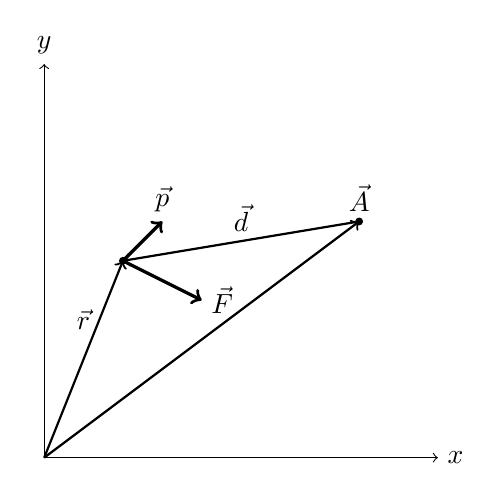
\begin{tikzpicture}[scale=5]
                \draw[<->] (0,1) |- (1,0);
                \node[above] at (0,1) {$y$};
                \node[right] at (1,0) {$x$};

                \draw[->,thick] (0,0) -- (0.2,0.5);
                \fill (0.2,0.5) circle [radius=0.01];
                \node[above] at (0.1,0.3) {$\vec{r}$};
                \draw[<->,very thick] (0.3,0.6) -- (0.2,0.5) -- (0.4,0.4);
                \node[above] at (0.3,0.6) {$\vec{p}$};
                \node[right] at (0.4,0.4) {$\vec{F}$};

                \draw[->,thick] (0,0) -- (0.8,0.6);
                \fill (0.8,0.6) circle [radius=0.01];
                \node[above] at (0.8,0.6) {$\vec{A}$};
                
                \draw[->,thick] (0.8,0.6) -- (0.2,0.5);
                \node[above] at (0.5,0.55) {$\vec{d}$};
            \end{tikzpicture}
        \end{figure}
        The angular momentum and torque relative to the origin are $\vec{L}=\vec{r}\times\vec{p}$ and $\vec{\tau}=\vec{r}\times\vec{F}$ like before, but what are the angular momentum and torque relative to the point $\vec{A}$?
        The radius vector or lever arm is now the vector $\vec{d}$ between the points $\vec{A}$ and $\vec{r}$, i.e.
        \begin{align}
            \vec{L}_{\vec{A}}&=\vec{d}\times\vec{p}\\
            &=(\vec{r}-\vec{A})\times\vec{p}\\
            \vec{\tau}_{\vec{A}}&=\vec{d}\times\vec{F}\\
            &=(\vec{r}-\vec{A})\times\vec{F}.
        \end{align}
        \begin{example}
            Consider a \qty{2}{\kilogram} particle at $y=\qty{3}{\meter}$ moving to the right with velocity $\vec{v}=\qty{5}{\meter\per\second}\ihat$.
            What is its angular momentum relative to the origin and relative to the point $\vec{A}=\qty{3}{\meter}\jhat$.
            \begin{figure}[H]
                \centering
                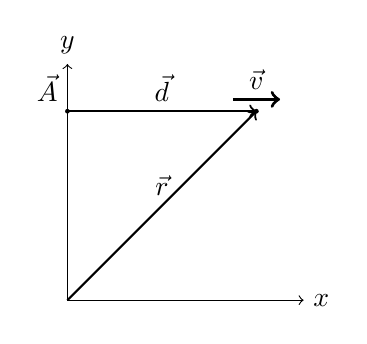
\begin{tikzpicture}[scale=3]
                    \draw[<->] (0,1) |- (1,0);
                    \node[above] at (0,1) {$y$};
                    \node[right] at (1,0) {$x$};

                    \fill (0,0.8) circle [radius=0.01];
                    \node[above left] at (0,0.8) {$\vec{A}$};

                    \fill (0.8,0.8) circle [radius=0.01];
                    \draw[->,very thick] (0.7,0.85) -- (0.9,0.85);
                    \node[above] at (0.8,0.85) {$\vec{v}$};

                    \draw[->,thick] (0,0.8) -- (0.8,0.8);
                    \node[above] at (0.4,0.8) {$\vec{d}$};
                    \draw[->,thick] (0,0) -- (0.8,0.8);
                    \node[above] at (0.4,0.4) {$\vec{r}$};
                \end{tikzpicture}
            \end{figure}
            The position vector is $\vec{r}=x\ihat+\qty{3}{\meter}\jhat$ and the radius vector relative to $\vec{A}$ is $\vec{d}=x\ihat$.
            The momentum vector is $\vec{p}=mv_x\ihat=\qty{10}{\kilogram\meter\per\second}$, so the angular momentum relative to the origin is
            \begin{align}
                \vec{L}&=\vec{r}\times\vec{p}=\begin{vmatrix}
                    \ihat & \jhat & \khat \\
                    x & 3 & 0 \\
                    10 & 0 & 0
                \end{vmatrix}\\
                &=-\qty{30}{\kilogram\meter\squared\per\second}\khat,
            \end{align}
            at the angular momentum relative to $\vec{A}$ is
            \begin{align}
                \vec{L}_{\vec{A}}&=\vec{d}\times\vec{p}=\begin{vmatrix}
                    \ihat & \jhat & \khat \\
                    x & 0 & 0 \\
                    10 & 0 & 0
                \end{vmatrix}\\
                &=0.
            \end{align}
            This makes sense because relative to $\vec{A}$ the motion is radial so there is no lever arm.
        \end{example}
        \begin{example}
            Let's now look at a familiar example, uniform circular motion.
            First, what is the angular momentum relative to the origin for a particle travelling with angular speed $\omega$?

            \paragraph{}
            Working in polar coordinates, the radius vector is $\vec{r}=r\uvec{r}$ and the velocity vector is $\vec{v}=r\omega\uvec{\theta}$.
            Then the angular momentum is $\vec{L}=r\uvec{r}\times mr\omega\uvec{\theta}=mr^2\omega\khat$.
            This is a constant, which we know to be the case since the centripetal force is a central force.

            \paragraph{}
            Now, suppose the particle is moving around a circle at $y=h$.
            What is the angular momentum relative to the origin?
            % TODO: include diagram for this

            \paragraph{}
            The position vector is now given by $\vec{r}=r\uvec{r}+h\khat$, so the angular momentum becomes
            \begin{align}
                \vec{L}&=m\begin{vmatrix}
                    \uvec{r} & \uvec{\theta} & \khat \\
                    r & 0 & h \\
                    0 & r\omega & 0
                \end{vmatrix}\\
                &=-mhr\omega\uvec{r}+mr^2\omega\khat.
            \end{align}
            The unit vector $\uvec{r}$ changes over time, so $\vec{L}$ is not constant (its magnitude is constant but its direction changes).
            This is because the centripetal force is no longer central relative to the origin.
        \end{example}

        \paragraph{}
        Torque is measured in $\unit{\newton\meter}$.
        This is dimensionally equivalent to Joules, but this does not mean that torque is a kind of energy.
        Energy is a scalar quantity, whereas torque is a vector, so they are really different things.

        \paragraph{}
        In linear dynamics, we have Newton's second law which states $\vec{F}=\dot{\vec{p}}$.
        We will now show that there is a rotational equivalent of Newton II that relates torque to angular momentum.
        Using the product rule to differentiate $\vec{L}$, we find
        \begin{align}
            \dv{\vec{L}}{t}&=\dv{}{t}(\vec{r}\times\vec{p})\\
            &=(\dot{\vec{r}}\times\vec{p})+(\vec{r}\times\dot{\vec{p}})\\
            &=\left(\frac{1}{m}\vec{p}\times\vec{p}\right)+(\vec{r}\times\vec{F})\\
            &=\vec{r}\times\vec{F}=\vec{\tau}.
        \end{align}
        This is the same calculation we did earlier for central forces.
        We now have a shortcut to prove that angular momentum is conserved under the influence of a central force.
        % TODO: add equation references
        Since central forces are always parallel to the radius vector, the torque is zero.
        \begin{equation}
            \vec{\tau}=\vec{r}\times F(r)\uvec{r}=0.
        \end{equation}
        Then using the angular equivalent of Newton II, $\dot{\vec{L}}=\vec{\tau}=0$.
        So central forces exert no torque and therefore angular momentum is conserved.

    \section{Torque and Angular Momentum for Systems of Particles}\label{sec:torque-and-angular-momentum-for-systems-of-particles}
        \paragraph{}
        In a system of many particles, each particle with a position $\vec{r}_i$ and momentum $\vec{p}_i$, the total angular momentum is the sum of each particle's angular momentum.
        \begin{equation}
            \vec{L}=\sum_i\vec{L}_i=\sum_i\vec{r}_i\times\vec{p}_i.
        \end{equation}
        If the particles are subject to some torques, their angular momenta will change.
        The total angular momentum changes as
        \begin{equation}
            \dv{\vec{L}}{t}=\sum_i\dv{\vec{L}_i}{t}=\sum_i\dv{}{t}(\vec{r}_i\times\vec{p}_i)=\sum_i\vec{r}_i\times\vec{F}_i=\sum_i\vec{\tau}_i.
        \end{equation}
        Let's look at the individual torques $\vec{\tau}_i$ more closely.
        The forces on each particle can be split into internal and external forces, $\vec{F}_i=\vec{F}_{i,\text{int}}+\vec{F}_{i,\text{ext}}$.
        Internal forces are those from other particles, so $\vec{F}_{i,\text{int}}$ can be written as
        \begin{equation}
            \vec{F}_{i,\text{int}}=\sum_{j\neq i}\vec{F}_{j\to i}.
        \end{equation}
        So the torques become
        \begin{align}
            \sum_i\vec{\tau}_i&=\sum_i\vec{r}_i\times\left(\sum_{j\neq i}\vec{F}_{j\to i}+\vec{F}_{i,\text{ext}}\right)\\
            &=\sum_i\sum_{j\neq i}\vec{r}_i\times\vec{F}_{j\to i}+\sum_i\vec{r}_i\times\vec{F}_{i,\text{ext}}.
        \end{align}
        Looking at the first term more closely, we can use a similar argument to back in chapter~\ref{chap:linear-momentum} to show that it is zero.
        % TODO: reference specific equation
        The sum will pairs of terms of the form $\vec{r}_i\times\vec{F}_{j\to i}+\vec{r}_j\times\vec{F}_{i\to j}$.
        By Newton III, these two forces are equal and opposite, $\vec{F}_{j\to i}=-\vec{F}_{i\to j}$, so the pair of terms becomes
        \begin{align}
            \vec{r}_i\times\vec{F}_{j\to i}+\vec{r}_j\times\vec{F}_{i\to j}&=\vec{r}_i\times\vec{F}_{j\to i}-\vec{r}_j\times\vec{F}_{j\to i}\\
            &=(\vec{r}_i-\vec{r}_j)\times\vec{F}_{j\to i}.
        \end{align}
        The vector $\vec{r}_i-\vec{r}_j$ is a vector which points from particle $j$ to particle $i$, which is parallel to the force $\vec{F}_{j\to i}$, therefore the whole sum is zero.
        Therefore the contribution to the torques comes \textit{only} from the external forces.
        Internal forces do \textit{not} contribute to the change in angular momentum.
        \begin{equation}
            \dot{\vec{L}}=\sum_i\vec{\tau}_i=\sum_i\vec{r}_i\times\vec{F}_{i,\text{ext}}.
        \end{equation}

        \paragraph{}
        Is $\dot{\vec{L}}=\tau_\text{ext}$?
        Only in two situations: when we consider the torque about the origin of an inertial frame of reference, and when we consider the torque about the centre of mass (even if the centre of mass frame is \textit{not} inertial).
        % TODO: prove this
        This is very important because it allows us to use the angular equivalent of Newton II in many situations.
        For example, if we are analysing a rigid body rolling down a hill, we can measure the angular momentum and torque from the centre of mass then we can still use $\dot{\vec{L}}=\vec{\tau}$.

    \section{Dynamics of Rigid Bodies}\label{sec:dynamics-of-rigid-bodies}
        \paragraph{}
        As stated in chapter~\ref{chap:angular-motion}, rigid bodies are distinguished by the fact that all mass elements have the same angular velocity $\omega$.
        % TODO: insert figure, rigid body rotation
        Each mass element is therefore moving in circles with speed $v_i=R_i\omega$, where $R_i$ is the distance from the axis of rotation.
        The smart choice for a coordinate system would be to align the $z$-axis with the axis of rotation and use cylindrical coordinates $(R,\phi,z)$, but let's look at the angular momentum in cartesian coordinates.
        The velocity of a mass element (assuming that the rigid body has no linear motion) is $\vec{v}_i=v_{x,i}\ihat+v_{y,i}\jhat=-\omega y_i\ihat+\omega x_i\jhat$.
        Then the total angular momentum is
        \begin{align}
            \vec{L}=\sum_i\vec{L}_i&=\sum_i\vec{r}_i\times m_i\vec{v_i}\\
            &=\sum_i m_i\begin{vmatrix}
                \ihat & \jhat & \khat \\
                x_i & y_i & z_i \\
                -\omega y_i & \omega x_i & 0
            \end{vmatrix}\\
            &=\sum_i m_ix_iz_i\omega\ihat+\sum_i m_iy_iz_i\omega\jhat+\sum_i m_i(x_i^2+y_i^2)\omega\khat.
        \end{align}
        The last term can be simplified to $\sum_i m_iR_i^2\omega\khat=I_z\omega\khat$ where $I_z$ is the moment of inertia about the $z$ axis.
        The first two terms are the \textbf{products of inertia} multiplied by $\omega$.
        % TODO: do this in cylindrical coordinates
        In the case where the products of inertia are zero, we have
        \begin{equation}
            \vec{L}=I_z\omega\khat,
        \end{equation}
        and the object is rotating around a \textbf{principle axis}.

        \paragraph{}
        Assuming this angular momentum is measured from the centre of mass of the rigid body, we can use $\vec{\tau}=\dot{\vec{L}}$ to get
        % TODO: is it valid if angular momentum is measured from the origin
        \begin{equation}
            \vec{\tau}=\dot{\vec{L}}=I\dot{\omega}\khat=I\alpha\khat.
        \end{equation}
        This is an angular analogue of Newton II where moment of inertia takes the place of mass.
        This derivation has also implicitly assumed that the torque is being applied around the axis of rotation and hence the direction of $\vec{L}$ does not change.
        A torque in another direction would change the direction of angular momentum, which leads to \textit{precession}
        In the case of constant torque around the axis of rotation, the equation above implies that $\alpha$ is constant, which means we can use the angular SUVAT equations from chapter~\ref{chap:angular-motion} to describe the motion. 
        \begin{example}
            Consider two connected masses on a massless pulley with $m_1>m_2$.
            Suppose the system starts from rest and assume the string is massless, inextensible, and lies vertically.
            Find an expression for the magnitude of acceleration of the masses.
            % TODO: include diagram for this
            To do this, we have to analyse the forces acting on the blocks and also the torques acting on the pulley.
            % TODO: complete this example
        \end{example}

        % TODO: discuss angular equivalent of impulse momentum theorem

    \section{Rolling Motion}\label{sec:rolling-motion}
        \paragraph{}
        One of the most familiar examples of torques in everyday life are rolling objects.
        Rolling motion is a superposition of a rotation about the centre of mass and a translation.
        In this section we will study \textbf{rolling without slipping}, which is the easiest type of rolling motion to analyse.
        We will also only look at circular rigid objects for now (wheels, balls, cylinders).
        \begin{figure}[H]
            \centering
            \begin{tikzpicture}[scale=1.5]
                \draw (-3,0) -- (3,0);
                \draw (0,1) circle [radius=1];
                \begin{scope}[shift={(0,1)}]
                    \draw[->,dashed] (0,0) -- (120:1);
                    \node[above right] at (120:0.5) {$R$};    
                \end{scope}
                
                \draw[->,thick] (0,1) -- (0.5,1);
                \node[above] at (0.25,1) {$\vec{v}_\text{COM}$};
                \draw[->,thick] (0,0) -- (-0.5,0);
                \node[below] at (-0.25,0) {$\vec{v}_\text{rim}$};
            \end{tikzpicture}
        \end{figure}
        In this case, we have that the contact point with the ground has \textit{zero} instantaneous velocity.
        For a circular rolling object, we can write
        \begin{equation}
            v_\text{COM}+v_\text{rim}=v_\text{COM}-R\omega=0.
        \end{equation}
        This implies that
        \begin{equation}
            v_\text{COM}=R\omega,
        \end{equation}
        which makes sense when we realise that for a circle that is rolling without slipping, its total distance travelled is $s=R\theta$ so $v_\text{COM}=\dot{s}=R\omega$.

        \paragraph{}
        For a disc (or a cylinder), its moment of inertia while rolling is $\frac{1}{2}mR^2$.
        % TODO: reference last chapter
        Then its total kinetic energy is
        \begin{align}
            K&=\frac{1}{2}mv_\text{COM}^2+\frac{1}{2}I\omega^2\\
            &=\frac{1}{2}mv_\text{COM}^2+\frac{1}{4}(mR^2)\left(\frac{v_\text{COM}}{R}\right)^2\\
            &=\frac{1}{2}mv_\text{COM}^2+\frac{1}{4}mv_\text{COM}^2=\frac{3}{4}mv_\text{COM}^2.
        \end{align}
        So the rotational energy is half of its translational energy, or to put it another way a third of its kinetic energy is stored in the rotational motion.

        \paragraph{}
        Let's look at the forces and torques involved in rolling.
        On a flat surface, if we have $a_\text{COM}=0$ then $\alpha=a/R=0$.
        This implies that the torque about the centre of mass is zero which means no force is acting on the rim of the object.
        All this is to say that there is no tendency to slide.
        If $a_\text{COM}\neq 0$, then there is a torque about the centre of mass and therefore there is a force.
        This must be a friction force, specifically static friction in the case of rolling without slipping.
        Thus we cannot have rolling without friction!

        \paragraph{}
        Which way does the static friction point?
        We are used to having static friction point to the left if the object is moving to the right, but there is a subtle gotcha here.
        In the case of rolling motion, the contact point wants to slip to the left, which means the static friction force must point to the right.
        On an incline, the weight does not exert a torque because it acts on the centre of mass, and the normal force does not exert a torque because it acts parallel to the radius vector.
        The only force which exerts a torque is the static friction, so $\tau_{f_s}=I\alpha$.
        \begin{example}
            A disc is rolling down an inclined plane.
            Find an expression for its acceleration.
            \begin{figure}[H]
                \centering
                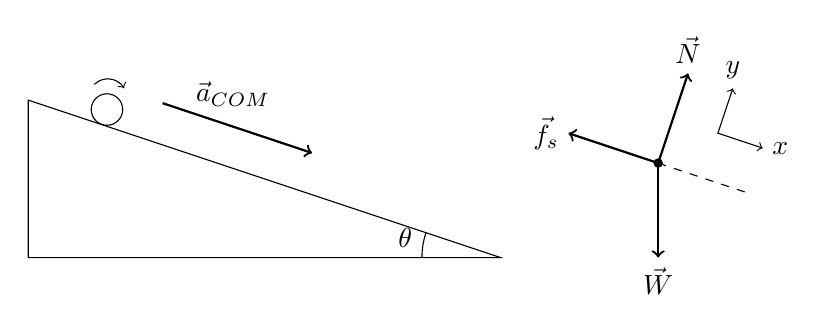
\begin{tikzpicture}[scale=2]
                    \draw (0,0) -- (3,0) -- (0,1) -- cycle;
                    \draw (0.5,0.94) circle [radius=0.1];
                    \draw (2.5,0) arc [radius=0.5, start angle=180, end angle=161.57];
                    \node[above left] at (2.5,0) {$\theta$};

                    \draw[->] (0.42,1.1) arc [radius=0.12, start angle=135, end angle=30];
                    \draw[->,thick,rotate=-18.43,shift={(0.5,1.2)}] (0,0) -- (1,0);
                    \node[above] at (1.3,0.9) {$\vec{a}_\text{COM}$};

                    \begin{scope}[shift={(4,0.6)},scale=0.6]
                        \fill (0,0) circle [radius=0.05];
                        \draw[->,thick] (0,0) -- (0,-1);
                        \node[below] at (0,-1) {$\vec{W}$};
                        \begin{scope}[rotate=-18.43]
                            \draw[->,thick] (0,0) -- (-1,0);
                            \node[left] at (-1,0) {$\vec{f}_s$};
                            \draw[->,thick] (0,0) -- (0,1);
                            \node[above] at (0,1) {$\vec{N}$};
                            \draw[dashed] (0,0) -- (1,0);

                            \begin{scope}[shift={(0.5,0.5)},scale=0.5]
                                \draw[<->] (0,1) |- (1,0);
                                \node[above] at (0,1) {$y$};
                                \node[right] at (1,0) {$x$};
                            \end{scope}
                        \end{scope}
                    \end{scope}
                \end{tikzpicture}
            \end{figure}
            
            \paragraph{}
            Looking at the forces in the $x$ direction, we get
            \begin{align}
                \sum F_x=m a_\text{COM}&=\abs{\vec{W}}\sin\theta-\abs{\vec{f}_s}\\
                &=mg\sin\theta-f_s.
            \end{align}
            Now we need to find an expression for the magnitude of static friction $f_s$, which we can do by analysing the torques.
            Since the only force which exerts a torque is static friction, we have $\tau_{f_s}=Rf_s=I\alpha$.
            So using the moment of inertia for a disc $\frac{1}{2}mR^2$ and substituting $\alpha=a_\text{COM}/R$, we get
            \begin{equation}
                f_s=\frac{I a_\text{COM}}{R^2}=\frac{1}{2}ma_\text{COM}.
            \end{equation}
            Substituting this into the equation above, we get
            \begin{align}
                ma_\text{COM}&=mg\sin\theta-\frac{1}{2}ma_\text{COM}\\
                &\implies a_\text{COM}=\frac{2}{3}g\sin\theta.
            \end{align}
            This result is somewhat interesting, the acceleration does not depend on the mass or radius of the disc, only the angle of the plane.
            % TODO: compare to a block sliding down an incline plane
            However, the acceleration does depend on the distribution of mass within the rolling object, i.e. the moment of inertia.
            If we had left the moment of inertia unspecified, we would get
            \begin{equation}
                a_\text{COM}=\frac{mg\sin\theta}{\frac{I}{R^2}+m}.
            \end{equation}
            This is valid for all circular rolling objects.
            As we have seen, the moment of inertia for most circular objects is proportional to $mR^2$, leading to a simplification with a different constant multiplying $g\sin\theta$.
        \end{example}
        % TODO: add example of sweet spot to hit a cue ball for perfect rolling
        % TODO: rolling cylinder along a flat plane and falling yo-yo as exersises, answers are very similar

    \section{Static Equilibrium}\label{sec:static-equilibrium}
        \paragraph{}
        In the net force and the net torque on a rigid body are both 0, then it is in \textbf{static equilibrium}.
        % TODO: include discussion of whether objects can be rotating in static equilibrium
        % TODO: include discussion about how static equilibrium implies net torque is zero in ALL inertial reference frames
        \begin{eqnarray}
            \sum_i\vec{F}_i=0\quad\text{and}\quad\sum_i\vec{\tau}_i=0.
        \end{eqnarray}
        Note that we are free to choose any point as the origin to make finding the net torqe easier.
        \begin{example}
            Consider a beam of mass 10kg and length 4m.
            It sits on a fulcrum placed 1m from one end of the beam, and is supported from the other end by a string.
            Find the tension in the string and the force of the beam on the fulcrum.
            % TODO: complete this example
        \end{example}
        \begin{example}
            A ladder weighing 10kg rests on a smooth wall.
            Find the the static friction force between the floor and the ladder.
            % TODO: complete this example
        \end{example}
        \begin{example}
            Consider a sign hanging from a bar attached to a wall supported by a string.
            Find the force between the bar and the wall.
            % TODO: complete this example
        \end{example}

\end{document}
